\documentclass[12pt,a4paper]{report}

% ============================================================
% PACKAGES
% ============================================================
\usepackage[utf8]{inputenc}
\usepackage[T1]{fontenc}
\usepackage[french]{babel}
\usepackage{geometry}
\geometry{top=2.5cm, bottom=2.5cm, left=2.5cm, right=2.5cm}

% Police Times New Roman
\usepackage{mathptmx}

\usepackage{graphicx}
\graphicspath{{./}{pics/}}
\usepackage{float}
\usepackage{caption}
\usepackage{subcaption}
\usepackage{xcolor}
\definecolor{darkblue}{RGB}{20,50,100}
\definecolor{lightblue}{RGB}{220,230,245}
\definecolor{darkgreen}{RGB}{30,80,30}

\usepackage{amsmath}
\usepackage{setspace}
\onehalfspacing

\usepackage{array}
\usepackage{booktabs}
\usepackage{tabularx}
\usepackage{longtable}

% TikZ pour diagrammes UML et illustrations
\usepackage{tikz}
\usetikzlibrary{shapes,arrows,positioning,calc,shadows,arrows.meta,fit}

% Listings pour le code source Kotlin
\usepackage{listings}
\lstdefinelanguage{Kotlin}{
  keywords={fun, val, var, if, else, when, while, for, return, class, override, import, package, by, remember, true, false, null, in, is, as, it, this, super, object, companion, data, sealed, enum, interface, abstract, open, inner, out, lateinit, const, suspend},
  keywordstyle=\color{darkblue}\bfseries,
  ndkeywords={Composable, Preview, LaunchedEffect, mutableStateOf, Box, Column, Row, Text, Button, Spacer, Modifier, Color, AlertDialog, Switch, Checkbox, OutlinedTextField},
  ndkeywordstyle=\color{darkgreen}\bfseries,
  sensitive=true,
  comment=[l]{//},
  morecomment=[s]{/*}{*/},
  commentstyle=\color{gray}\itshape,
  string=[b]",
  stringstyle=\color{red!70!black},
}
\lstset{
  language=Kotlin,
  basicstyle=\ttfamily\scriptsize,
  numberstyle=\tiny\color{gray},
  numbers=left,
  frame=single,
  breaklines=true,
  showstringspaces=false,
  tabsize=4,
  captionpos=b,
  xleftmargin=1.5em,
  framexleftmargin=1.5em,
  backgroundcolor=\color{lightblue!30},
  rulecolor=\color{darkblue},
}

% En-tetes et pieds de page
\usepackage{fancyhdr}
\setlength{\headheight}{15pt}
\pagestyle{fancy}
\fancyhf{}
\fancyhead[L]{\small Projet Paddle Pong -- 4IIRG3}
\fancyhead[R]{\small\nouppercase{\leftmark}}
\fancyfoot[C]{\thepage}
\renewcommand{\headrulewidth}{0.4pt}
\renewcommand{\chaptermark}[1]{\markboth{Chapitre \thechapter\ -- #1}{}}

% Titres en noir
\usepackage{titlesec}
\titleformat{\chapter}[display]
  {\normalfont\huge\bfseries\color{black}}
  {\chaptertitlename\ \thechapter}{18pt}{\Huge}
\titlespacing*{\chapter}{0pt}{0pt}{20pt}
\titleformat{\section}{\normalfont\Large\bfseries\color{black}}{\thesection}{1em}{}
\titleformat{\subsection}{\normalfont\large\bfseries\color{black}}{\thesubsection}{1em}{}
\titleformat{\subsubsection}{\normalfont\normalsize\bfseries\color{black}}{\thesubsubsection}{1em}{}

\usepackage[colorlinks=true,
            linkcolor=darkblue,
            urlcolor=darkblue,
            citecolor=darkblue,
            pdftitle={Rapport de Projet - Paddle Pong Mini Game},
            pdfauthor={Nizar El Idrysy, Mohammed Lamrani Hnini, Hidaya Similla}]{hyperref}

\usepackage{mdframed}
\usepackage{enumitem}

% ============================================================
% DEBUT DU DOCUMENT
% ============================================================
\begin{document}

% ------------------------------------------------------------
% PAGE DE GARDE
% ------------------------------------------------------------
\begin{titlepage}
    \begin{tikzpicture}[remember picture, overlay]
        \fill[green!40!black] (current page.south east) -- ++(-6,0) -- ++(6,6) -- cycle;
        \node[rotate=45, text=white, font=\bfseries\Huge] at ([shift={(-1.8, 1.8)}]current page.south east) {4IIR};
    \end{tikzpicture}
    \begin{tikzpicture}[remember picture, overlay]
        \node[anchor=north west, xshift=1.5cm, yshift=-1.5cm] at (current page.north west) {
            
\includegraphics[width=6cm, height=3.5cm, keepaspectratio]{logoEmsi.png}
        };
    \end{tikzpicture}
    \begin{center}
        \vspace*{3.5cm}
        \textsc{\Large \'Ecole Marocaine des Sciences de l'Ing\'enieur de Tanger}\\[0.1cm]
        \vspace{0.8cm}
        {\Huge \textbf{RAPPORT DE PROJET}}
        \vspace{0.6cm} \\
        {\large 2\textsuperscript{\`eme} Ann\'ee -- Cycle d'ing\'enieur (4IIR)}
        \vspace{0.4cm} \\
        {\large Mati\`ere : D\'eveloppement Mobile (Android)}
        \vspace{0.8cm} \\
        {\textbf{Intitul\'e du Projet :}}
        \vspace{0.8cm}
        \noindent\fbox{
            \begin{minipage}{\dimexpr\textwidth-2\fboxsep-2\fboxrule\relax}
                \centering
                \vspace{0.8cm}
                {\Huge \textbf{PADDLE PONG}}\\[0.4cm]
                {\Large \textbf{Conception et D\'eveloppement d'un Mini-Jeu\\
                Mobile Android avec Jetpack Compose}}
                \vspace{0.8cm}
            \end{minipage}
        }
        \vspace{2.2cm}
        \begin{minipage}{0.45\textwidth}
            \begin{flushleft}
                \textbf{R\'ealis\'e par :} \\
                \vspace{0.2cm}
                EL IDRYSY Nizar \\
                LAMRANI HNINI Mohammed \\
                SIMILLA Hidaya \\
            \end{flushleft}
        \end{minipage}
        \hfill
        \begin{minipage}{0.50\textwidth}
            \begin{flushright}
                \textbf{Encadr\'e par :} \\
                \vspace{0.2cm}
                M. BENTAYEB Youness \textit{(EMSI)}\\
            \end{flushright}
        \end{minipage}

        \vfill
        \textbf{Novembre 2026} \\
        \textbf{Ann\'ee Universitaire 2026-2027}
    \end{center}
\end{titlepage}

% ------------------------------------------------------------
% PAGES PRELIMINAIRES
% ------------------------------------------------------------
\pagenumbering{roman}
\setcounter{page}{1}
\pagestyle{plain}

% --- REMERCIEMENTS ---
\chapter*{Remerciements}
\addcontentsline{toc}{chapter}{Remerciements}

Avant d'entamer la pr\'esentation de ce rapport de projet, nous tenons \`a exprimer notre profonde gratitude et nos sinc\`eres remerciements \`a toutes les personnes qui ont contribu\'e au bon d\'eroulement de ce travail.

Nous souhaitons adresser nos remerciements les plus chaleureux \`a notre encadrant p\'edagogique, \textbf{M. Youness Bentayeb}, pour sa disponibilit\'e, ses orientations pr\'ecieuses et son suivi m\'ethodologique tout au long de la r\'ealisation de ce projet. Ses conseils techniques sur le d\'eveloppement mobile Android et l'architecture applicative ont \'et\'e d\'eterminants pour la r\'eussite de ce travail.

Nos remerciements s'adressent \'egalement \`a l'ensemble du corps professoral et administratif de l'\textbf{\'Ecole Marocaine des Sciences de l'Ing\'enieur (EMSI Tanger)}, en particulier les enseignants du d\'epartement Informatique et R\'eseaux, pour l'excellence de la formation dispens\'ee et les connaissances fondamentales transmises en programmation orient\'ee objet, en architecture logicielle et en d\'eveloppement mobile.

Enfin, nous remercions nos familles et nos coll\`egues de la promotion \textbf{4IIRG3} pour leur soutien et leurs encouragements constants.

\newpage

% --- RESUME ---
\chapter*{R\'esum\'e}
\addcontentsline{toc}{chapter}{R\'esum\'e}

Dans le cadre du module de D\'eveloppement Mobile dispens\'e en deuxi\`eme ann\'ee du cycle d'ing\'enieur en Ing\'enierie Informatique et R\'eseaux \`a l'EMSI Tanger, notre \'equipe a con\c{c}u et d\'evelopp\'e un mini-jeu mobile Android intitul\'e \textbf{Paddle Pong}. Ce projet a \'et\'e r\'ealis\'e enti\`erement en \textbf{Kotlin} en exploitant le framework d\'eclaratif \textbf{Jetpack Compose}, le paradigme d'interface utilisateur moderne recommand\'e par Google pour le d\'eveloppement Android.

L'application propose une exp\'erience de jeu de type \textit{Pong} dans laquelle le joueur contr\^ole une raquette horizontale pour intercepter une balle rebondissante et accumuler des points. Le projet int\`egre un \'ecran de configuration (saisie du pseudonyme, choix de la vitesse, mode sombre), un moteur de jeu bas\'e sur une boucle de coroutines Kotlin, une gestion de collisions et un syst\`eme de score avec dialogue de fin de partie.

Ce rapport d\'etaille l'ensemble du cycle de d\'eveloppement : contexte et \'etude pr\'eliminaire, conception g\'en\'erale avec mod\'elisation UML, et r\'ealisation technique incluant l'impl\'ementation du code source, les captures d'\'ecran, les tests et l'analyse critique du projet.

\medskip
\noindent\textbf{Mots-cl\'es :} Android, Kotlin, Jetpack Compose, D\'eveloppement mobile, Mini-jeu, Pong, Coroutines, Architecture d\'eclarative, Material Design 3, Android Studio.

\newpage

% --- ABSTRACT ---
\chapter*{Abstract}
\addcontentsline{toc}{chapter}{Abstract}

As part of the Mobile Development course in the second year of the Computer Engineering and Networks program at EMSI Tangier, our team designed and developed an Android mobile mini-game titled \textbf{Paddle Pong}. The project was entirely built in \textbf{Kotlin} using the \textbf{Jetpack Compose} declarative UI framework, Google's modern recommended approach for Android user interface development.

The application offers a Pong-style gaming experience where the player controls a horizontal paddle to intercept a bouncing ball and accumulate points. The project incorporates a setup screen (player name input, speed selection, dark mode toggle), a game engine powered by Kotlin coroutine loops, collision detection logic, and a scoring system with an end-of-game dialog.

This report covers the complete development lifecycle: project context and preliminary study, general design with UML modeling, and technical implementation including source code walkthrough, application screenshots, testing procedures, and critical project analysis.

\medskip
\noindent\textbf{Keywords:} Android, Kotlin, Jetpack Compose, Mobile Development, Mini-game, Pong, Coroutines, Declarative Architecture, Material Design 3, Android Studio.

\newpage

% --- TABLES DES MATIERES, FIGURES, TABLEAUX ---
\tableofcontents
\newpage
\listoffigures
\addcontentsline{toc}{chapter}{Liste des figures}
\newpage
\listoftables
\addcontentsline{toc}{chapter}{Liste des tableaux}
\newpage

% --- LISTE DES ABREVIATIONS ---
\chapter*{Liste des abr\'eviations}
\addcontentsline{toc}{chapter}{Liste des abr\'eviations}

\begin{center}
\begin{tabular}{p{3cm} p{11.5cm}}
\toprule
\textbf{Abr\'eviation} & \textbf{Signification} \\
\midrule
ADB   & Android Debug Bridge \\
API   & Application Programming Interface \\
APK   & Android Package Kit \\
AVD   & Android Virtual Device (\'Emulateur) \\
CdC   & Cahier des Charges \\
dp    & Density-independent Pixels (unit\'e de mesure Android) \\
FPS   & Frames Per Second (Images par seconde) \\
IDE   & Integrated Development Environment \\
JVM   & Java Virtual Machine \\
KSP   & Kotlin Symbol Processing \\
MD3   & Material Design 3 (Material You) \\
MVC   & Model--View--Controller \\
MVVM  & Model--View--ViewModel \\
SDK   & Software Development Kit \\
sp    & Scale-independent Pixels (unit\'e typographique Android) \\
UI    & User Interface (Interface Utilisateur) \\
UML   & Unified Modeling Language \\
UX    & User Experience (Exp\'erience Utilisateur) \\
XML   & Extensible Markup Language \\
\bottomrule
\end{tabular}
\end{center}

\newpage

% ============================================================
% CORPS DU RAPPORT
% ============================================================
\pagenumbering{arabic}
\setcounter{page}{1}
\pagestyle{fancy}

% ------------------------------------------------------------
% INTRODUCTION GENERALE
% ------------------------------------------------------------
\chapter*{Introduction G\'en\'erale}
\addcontentsline{toc}{chapter}{Introduction G\'en\'erale}
\markboth{Introduction G\'en\'erale}{}

Le d\'eveloppement d'applications mobiles constitue aujourd'hui l'une des comp\'etences fondamentales attendues d'un ing\'enieur en informatique. Avec plus de 3,5 milliards d'appareils Android actifs dans le monde en 2026~\cite{statcounter}, la plateforme Android demeure l'\'ecosyst\`eme mobile dominant et repr\'esente un terrain d'apprentissage incontournable pour les \'etudiants en g\'enie logiciel.

Dans le cadre du module de D\'eveloppement Mobile dispens\'e par \textbf{M. Youness Bentayeb} en 4\textsuperscript{\`eme} ann\'ee du cycle d'ing\'enieur (4IIR) \`a l'\textbf{EMSI Tanger}, notre \'equipe compos\'ee de \textbf{Nizar El Idrysy}, \textbf{Mohammed Lamrani Hnini} et \textbf{Hidaya Similla} a \'et\'e charg\'ee de concevoir et de d\'evelopper un mini-jeu mobile Android. L'objectif p\'edagogique de ce projet est double : d'une part, ma\^itriser les fondamentaux du d\'eveloppement Android moderne avec \textbf{Kotlin} et \textbf{Jetpack Compose}, et d'autre part, appliquer une d\'emarche de g\'enie logiciel compl\`ete (analyse, conception, impl\'ementation et tests) sur un projet concret.

Le jeu retenu, \textbf{Paddle Pong}, est inspir\'e du classique \textit{Pong} (Atari, 1972), consid\'er\'e comme le premier jeu vid\'eo commercial \`a succ\`es. Notre version mobile met le joueur aux commandes d'une raquette qu'il d\'eplace horizontalement pour intercepter une balle qui rebondit sur les parois d'un terrain de jeu. Chaque interception r\'eussie rapporte un point, et la partie se termine lorsque la balle franchit le bas du terrain.

Ce choix de projet permet d'aborder des probl\'ematiques techniques vari\'ees : la gestion d'\'etat r\'eactif avec Compose, l'animation par boucle de coroutines, la d\'etection de collisions en 2D, l'ergonomie d'une interface de jeu tactile et l'application des principes de Material Design 3.

Pour rendre compte de cette r\'ealisation, le pr\'esent rapport s'articule autour de trois chapitres compl\'ementaires. Le \textbf{premier chapitre} pr\'esente le contexte g\'en\'eral du projet, le cadre acad\'emique et la planification. Le \textbf{deuxi\`eme chapitre} formalise la conception g\'en\'erale et la mod\'elisation UML de l'application. Enfin, le \textbf{troisi\`eme chapitre} expose la r\'ealisation technique, les extraits de code cl\'es, les captures d'\'ecran de l'application, les tests de validation et l'analyse critique SWOT du projet.

\newpage

% ============================================================
% CHAPITRE 1 : CONTEXTE GENERAL DU PROJET ET ETUDE PRELIMINAIRE
% ============================================================
\chapter[Contexte et \'etude pr\'eliminaire]{Contexte g\'en\'eral du projet et \'etude pr\'eliminaire}

\section*{Introduction}
Ce premier chapitre d\'efinit le cadre g\'en\'eral du projet Paddle Pong. Il pr\'esente l'\'ecole d'accueil, le contexte p\'edagogique, le cahier des charges, la probl\'ematique trait\'ee, la planification des t\^aches et les objectifs assign\'es.

\section{Pr\'esentation de l'\'ecole d'accueil}
\subsection{Pr\'esentation g\'en\'erale de l'EMSI}
L'\textbf{\'Ecole Marocaine des Sciences de l'Ing\'enieur (EMSI)} est un \'etablissement priv\'e d'enseignement sup\'erieur fond\'e en 1986. L'EMSI est accr\'edit\'ee par le Minist\`ere de l'Enseignement Sup\'erieur et forme des ing\'enieurs dans des fili\`eres couvrant l'informatique, les r\'eseaux, le g\'enie civil et le g\'enie industriel. Le campus de Tanger, o\`u se d\'eroule notre formation, offre un environnement p\'edagogique moderne avec des laboratoires informatiques \'equip\'es.

\subsection{Fili\`ere Informatique et R\'eseaux (IIR)}
La fili\`ere \textbf{Ing\'enierie Informatique et R\'eseaux (IIR)} forme des ing\'enieurs polyvalents capables de concevoir, d\'evelopper et administrer des syst\`emes informatiques complexes. Le cursus couvre la programmation orient\'ee objet, les architectures logicielles, le d\'eveloppement web et mobile, les r\'eseaux et les syst\`emes distribu\'es.

Le module de \textbf{D\'eveloppement Mobile}, dispens\'e en 4\textsuperscript{\`eme} ann\'ee (4IIR), introduit les concepts fondamentaux de la programmation Android : cycle de vie des activit\'es, layouts, gestion d'\'etat, navigation et publication sur le Google Play Store.

\section{Contexte g\'en\'eral du projet}
\subsection{Pr\'esentation du projet}
Le projet \textbf{Paddle Pong} s'inscrit dans le cadre du module de D\'eveloppement Mobile. Il consiste \`a concevoir et impl\'ementer une application Android de type mini-jeu \textit{arcade}. L'application doit \^etre enti\`erement r\'ealis\'ee en Kotlin avec Jetpack Compose, sans d\'ependances externes lourdes, et doit fonctionner sur tout appareil Android \`a partir de l'API 24 (Android 7.0 Nougat).

\subsection{Cahier des charges (CdC)}
Le cahier des charges d\'efinit les sp\'ecifications suivantes :
\begin{itemize}
    \item \textbf{Terrain de jeu :} Rectangle de 280 $\times$ 300 dp (density-independent pixels).
    \item \textbf{Balle :} \'El\'ement carr\'e de 24 $\times$ 24 dp, position initiale \`a $(128, 20)$.
    \item \textbf{Raquette :} Rectangle de 72 $\times$ 12 dp, position initiale \`a $(104, 268)$.
    \item \textbf{D\'eplacement de la raquette :} Par pas discrets de 16 dp (gauche/droite), via deux boutons de contr\^ole.
    \item \textbf{Vitesse de la balle :} Trois niveaux s\'electionnables : Lent (65 ms), Normal (45 ms), Rapide (30 ms).
    \item \textbf{Score :} Incr\'ement\'e de 1 \`a chaque interception r\'eussie par la raquette.
    \item \textbf{Game Over :} D\'eclench\'e lorsque la balle d\'epasse le bas du terrain.
    \item \textbf{Fonctionnalit\'es suppl\'ementaires :} Saisie du pseudonyme du joueur, mode sombre, cr\'edits.
\end{itemize}

\section{Probl\'ematique}
Le d\'eveloppement d'un mini-jeu mobile en Jetpack Compose soul\`eve plusieurs d\'efis techniques :
\begin{enumerate}
    \item \textbf{Gestion de la boucle de jeu en environnement d\'eclaratif :} Contrairement aux frameworks imp\'eratifs traditionnels (Canvas avec \texttt{onDraw}), Compose fonctionne par recomposition r\'eactive. Il faut int\'egrer une boucle de mise \`a jour temporelle (game loop) sans bloquer le thread UI.
    \item \textbf{D\'etection de collisions en temps r\'eel :} La balle doit rebondir correctement sur les parois et la raquette, n\'ecessitant un algorithme de d\'etection de collision AABB (Axis-Aligned Bounding Box) ex\'ecut\'e \`a chaque tick.
    \item \textbf{Fluidit\'e et performance :} Garantir une animation fluide (absence de saccades) sur des appareils Android d'entr\'ee de gamme avec des d\'elais de rafra\^ichissement de 30 \`a 65 ms.
    \item \textbf{Ergonomie tactile :} Concevoir des contr\^oles de raquette intuitifs et r\'eactifs dans un contexte mobile tactile.
\end{enumerate}

\section{Planification du projet}
\subsection{M\'ethodologie de travail}
L'\'equipe a adopt\'e une m\'ethodologie agile simplifi\'ee, structur\'ee en sprints courts :
\begin{enumerate}
    \item \textbf{Sprint 1 -- Analyse et conception :} R\'edaction du cahier des charges, identification des besoins fonctionnels, cr\'eation des diagrammes UML et maquettes d'interface.
    \item \textbf{Sprint 2 -- Impl\'ementation du noyau :} D\'eveloppement de la boucle de jeu, de la gestion de la balle et de la raquette, et de la d\'etection de collisions.
    \item \textbf{Sprint 3 -- Interface et personnalisation :} Impl\'ementation de l'\'ecran de configuration, du mode sombre, du syst\`eme de score et du dialogue de fin de partie.
    \item \textbf{Sprint 4 -- Tests, correction et r\'edaction :} Tests fonctionnels sur \'emulateur et appareil physique, correction des bogues, r\'edaction du rapport.
\end{enumerate}

\section{Objectifs du projet}
Les objectifs op\'erationnels fix\'es sont :
\begin{itemize}
    \item Concevoir une application Android native fonctionnelle, enti\`erement en Jetpack Compose.
    \item Impl\'ementer un moteur de jeu 2D l\'eger avec boucle de mise \`a jour par coroutines.
    \item Offrir une interface utilisateur ergonomique, esth\'etique et conforme aux principes Material Design 3.
    \item D\'elivrer un APK install\'e et test\'e sur \'emulateur et sur appareil physique Android.
    \item Produire une documentation technique compl\`ete sous forme de rapport.
\end{itemize}

\section{Pr\'esentation g\'en\'erale de la solution propos\'ee}
La solution retenue repose sur une application mono-activit\'e (\texttt{MainActivity}) exploitant exclusivement Jetpack Compose pour le rendu de l'interface. Le jeu est impl\'ement\'e dans un composable unique (\texttt{PaddlePongApp}) qui g\`ere \`a la fois l'\'ecran de configuration et l'\'ecran de jeu via un syst\`eme de gestion d'\'etat r\'eactif. La boucle de jeu est port\'ee par une coroutine Kotlin lanc\'ee via \texttt{LaunchedEffect}, qui met \`a jour la position de la balle et d\'etecte les collisions \`a intervalles r\'eguliers.

\section*{Conclusion}
Ce chapitre a permis de cadrer le contexte p\'edagogique et technique du projet Paddle Pong, de pr\'esenter le cahier des charges et les d\'efis \`a relever. Le chapitre suivant pr\'esente la conception g\'en\'erale de l'application Paddle Pong.

\newpage

% ============================================================
% CHAPITRE 2 : CONCEPTION GENERALE
% ============================================================
\chapter{Conception g\'en\'erale}

\section*{Introduction}
Ce chapitre est d\'edi\'e \`a la conception g\'en\'erale de l'application Paddle Pong. Il d\'etaille l'analyse des besoins fonctionnels et non fonctionnels, l'architecture logicielle et la mod\'elisation UML du syst\`eme.

\section{Analyse des besoins}

\subsection{Identification des acteurs}
L'application interagit avec un acteur principal :
\begin{itemize}
    \item \textbf{Joueur :} L'utilisateur final de l'application. Il configure sa partie (pseudonyme, vitesse, th\`eme), contr\^ole la raquette pendant le jeu, consulte son score et d\'ecide de rejouer ou de revenir \`a l'\'ecran de configuration.
\end{itemize}

\subsection{Besoins fonctionnels}
L'application doit assurer les fonctionnalit\'es suivantes :
\begin{enumerate}
    \item \textbf{BF1 -- Configuration de la partie :} Le joueur peut saisir un pseudonyme (champ obligatoire non vide), s\'electionner la vitesse de la balle parmi trois niveaux et activer/d\'esactiver le mode sombre.
    \item \textbf{BF2 -- Boucle de jeu :} La balle se d\'eplace de mani\`ere continue avec rebond sur les parois et la raquette.
    \item \textbf{BF3 -- Contr\^ole de la raquette :} Deux boutons permettent de d\'eplacer la raquette par pas discrets vers la gauche et vers la droite, avec limitation aux bornes du terrain.
    \item \textbf{BF4 -- Scoring :} Le score est incr\'ement\'e de 1 \`a chaque collision balle--raquette.
    \item \textbf{BF5 -- Fin de partie :} Un dialogue \texttt{AlertDialog} affiche le score final avec deux options : \og Rejouer \fg{} et \og Terminer \fg{}.
    \item \textbf{BF6 -- Affichage des informations :} Le pseudonyme, le mode de vitesse et le score courant sont affich\'es en permanence pendant la partie.
    \item \textbf{BF7 -- Cr\'edits :} Un encart affiche les d\'eveloppeurs, l'encadrant et la date de cr\'eation.
\end{enumerate}

\subsection{Besoins non fonctionnels}
\begin{itemize}
    \item \textbf{Performance :} La boucle de jeu doit s'ex\'ecuter sans saccade perceptible, avec un d\'elai minimal de 30 ms entre chaque tick (soit environ 33 FPS au maximum).
    \item \textbf{Compatibilit\'e :} L'application doit fonctionner sur Android 7.0 (API 24) et versions sup\'erieures, couvrant ainsi plus de 97\% des appareils actifs~\cite{android_distribution}.
    \item \textbf{Ergonomie :} Les boutons de contr\^ole doivent \^etre suffisamment grands pour une utilisation tactile confortable.
    \item \textbf{Accessibilit\'e :} Le mode sombre doit offrir un contraste suffisant pour la lisibilit\'e.
\end{itemize}

\section{Sp\'ecification de la solution}

\subsection{Architecture g\'en\'erale de l'application}
L'application adopte une architecture \textbf{mono-activit\'e} conforme aux recommandations modernes de Google :

\begin{itemize}
    \item \textbf{Couche Pr\'esentation :} La \texttt{MainActivity} h\'eberge le contenu Compose via \texttt{setContent}. L'unique composable racine \texttt{PaddlePongApp()} g\`ere l'ensemble de l'interface.
    \item \textbf{Couche Logique m\'etier :} La logique de jeu (d\'eplacement de la balle, d\'etection de collisions, gestion du score) est int\'egr\'ee directement dans le composable via des variables d'\'etat r\'eactives et une coroutine \texttt{LaunchedEffect}.
    \item \textbf{Couche Donn\'ees :} L'\'etat de l'application est enti\`erement g\'er\'e en m\'emoire (pas de persistance locale), via des variables \texttt{mutableStateOf} encapsul\'ees dans des d\'el\'egu\'es \texttt{remember}.
\end{itemize}

\begin{figure}[H]
\centering
\begin{tikzpicture}[node distance=1.5cm, auto, >=stealth']
    \tikzstyle{layer} = [rectangle, draw, fill=lightblue!50, text width=10cm, text centered, minimum height=1.5cm, font=\small\bfseries]

    \node [layer, fill=orange!25] (ui) {Couche Pr\'esentation\\{\scriptsize \texttt{PaddlePongApp()} -- Composables Compose (Column, Box, Row, Text, Button)}};
    \node [layer, fill=lightblue!60, below=0.6cm of ui] (logic) {Couche Logique M\'etier\\{\scriptsize Game Loop (\texttt{LaunchedEffect}), Collisions AABB, Score, \'Etat r\'eactif}};
    \node [layer, fill=green!20, below=0.6cm of logic] (state) {Couche \'Etat (Donn\'ees en m\'emoire)\\{\scriptsize \texttt{mutableStateOf}: ballX, ballY, paddleX, score, isPlaying, isGameOver}};

    \draw [<->, thick] (ui) -- node[font=\tiny, right] {Recomposition} (logic);
    \draw [<->, thick] (logic) -- node[font=\tiny, right] {Lecture/\'Ecriture d'\'etat} (state);
\end{tikzpicture}
\caption{Architecture en couches de l'application Paddle Pong}
\label{fig:app_arch}
\end{figure}

\subsection{Dimensions et param\`etres du terrain de jeu}
Les dimensions du terrain et des \'el\'ements de jeu sont synth\'etis\'ees dans le tableau~\ref{tab:dimensions}.

\begin{table}[H]
\centering
\caption{Dictionnaire des dimensions et param\`etres du jeu (en dp)}
\label{tab:dimensions}
\begin{tabularx}{\textwidth}{lXl}
\toprule
\textbf{\'El\'ement} & \textbf{Description} & \textbf{Valeur} \\
\midrule
\texttt{fieldWidth} & Largeur du terrain de jeu & 280 dp \\
\texttt{fieldHeight} & Hauteur du terrain de jeu & 300 dp \\
\texttt{ballSize} & Dimension de la balle (carr\'e) & 24 dp \\
\texttt{initialBallX} & Position X initiale de la balle & 128 dp \\
\texttt{initialBallY} & Position Y initiale de la balle & 20 dp \\
\texttt{paddleWidth} & Largeur de la raquette & 72 dp \\
\texttt{paddleHeight} & Hauteur de la raquette & 12 dp \\
\texttt{initialPaddleX} & Position X initiale de la raquette & 104 dp \\
\texttt{paddleY} & Position Y fixe de la raquette & 268 dp \\
\texttt{paddleStep} & Pas de d\'eplacement de la raquette & 16 dp \\
\texttt{dx}, \texttt{dy} & Vitesse de la balle (par tick) & $\pm$4 dp \\
\bottomrule
\end{tabularx}
\end{table}

\section{Conception UML}
La conception de l'application Paddle Pong est formalis\'ee \`a travers trois diagrammes UML : le diagramme de cas d'utilisation, le diagramme de s\'equence et le diagramme d'activit\'e.

\subsection{Diagramme de cas d'utilisation}
Le diagramme de cas d'utilisation (figure~\ref{fig:uml_use_case}) d\'efinit le p\'erim\`etre fonctionnel de l'application et les interactions du joueur avec le syst\`eme.

\begin{figure}[H]
\centering
\begin{tikzpicture}[font=\scriptsize]
    % Systeme
    \draw[thick, darkblue] (0,0) rectangle (10,-9);
    \node[font=\bfseries\small, darkblue] at (5,0.3) {Syst\`eme : Paddle Pong};

    % Acteur
    \node[font=\small] at (-1.8,-4.5) {Joueur};
    \draw (-1.8,-3.5) circle (0.3);
    \draw (-1.8,-3.8) -- (-1.8,-4.6);
    \draw (-1.8,-4.0) -- (-2.3,-4.3);
    \draw (-1.8,-4.0) -- (-1.3,-4.3);
    \draw (-1.8,-4.6) -- (-2.2,-5.1);
    \draw (-1.8,-4.6) -- (-1.4,-5.1);

    % Cas d'utilisation
    \tikzstyle{usecase} = [ellipse, draw, fill=lightblue!40, text width=2.8cm, text centered, minimum height=0.9cm, font=\tiny]
    \node[usecase] (uc1) at (5,-0.9) {Saisir pseudonyme};
    \node[usecase] (uc2) at (5,-2.1) {Choisir vitesse de la balle};
    \node[usecase] (uc3) at (5,-3.3) {Activer mode sombre};
    \node[usecase] (uc4) at (5,-4.5) {Lancer la partie};
    \node[usecase] (uc5) at (5,-5.7) {D\'eplacer la raquette};
    \node[usecase] (uc6) at (5,-6.9) {Consulter le score};
    \node[usecase] (uc7) at (5,-8.1) {Rejouer / Terminer};

    % Relations
    \draw[-] (-1.5,-4.2) -- (uc1.west);
    \draw[-] (-1.5,-4.2) -- (uc2.west);
    \draw[-] (-1.5,-4.2) -- (uc3.west);
    \draw[-] (-1.5,-4.2) -- (uc4.west);
    \draw[-] (-1.5,-4.2) -- (uc5.west);
    \draw[-] (-1.5,-4.2) -- (uc6.west);
    \draw[-] (-1.5,-4.2) -- (uc7.west);
\end{tikzpicture}
\caption{Diagramme de cas d'utilisation de l'application Paddle Pong}
\label{fig:uml_use_case}
\end{figure}

Le tableau~\ref{tab:uc_description} d\'etaille la fiche descriptive formelle du cas d'utilisation principal \og Jouer une partie \fg{}.

\begin{table}[H]
\centering
\caption{Fiche descriptive du cas d'utilisation \og Jouer une partie \fg{}}
\label{tab:uc_description}
\begin{tabularx}{\textwidth}{lX}
\toprule
\textbf{Champ} & \textbf{Description d\'etaill\'ee} \\
\midrule
\textbf{Cas d'utilisation} & Jouer une partie de Paddle Pong \\
\textbf{Acteur principal} & Joueur \\
\textbf{Pr\'econditions} & 1. L'application est lanc\'ee et l'\'ecran de configuration est affich\'e.\\
                         & 2. Le joueur a saisi un pseudonyme valide (non vide).\\
                         & 3. Une vitesse de balle est s\'electionn\'ee. \\
\textbf{Sc\'enario nominal} & 1. Le joueur appuie sur \og Start Paddling! \fg{}.\\
                            & 2. L'\'ecran de jeu s'affiche avec le terrain, la balle et la raquette.\\
                            & 3. La balle commence \`a se d\'eplacer en diagonale.\\
                            & 4. Le joueur d\'eplace la raquette avec les boutons $<$ et $>$.\\
                            & 5. La balle rebondit sur les murs et la raquette ; le score augmente.\\
                            & 6. La balle d\'epasse le bas du terrain : Game Over.\\
                            & 7. Le dialogue affiche le score ; le joueur choisit \og Rejouer \fg{} ou \og Terminer \fg{}. \\
\textbf{Postconditions} & Le score est affich\'e. L'\'etat du jeu est r\'einitialis\'e. \\
\bottomrule
\end{tabularx}
\end{table}

\subsection{Diagramme de s\'equence}
Le diagramme de s\'equence (figure~\ref{fig:uml_sequence}) mod\'elise le processus chronologique d'une partie compl\`ete, depuis le lancement jusqu'\`a la fin de partie.

\begin{figure}[H]
\centering
\begin{tikzpicture}[font=\tiny, >=stealth']
    % Lifelines
    \node[rectangle, draw, fill=lightblue!50, minimum width=1.6cm, minimum height=0.6cm] (joueur) at (0,0) {\textbf{Joueur}};
    \node[rectangle, draw, fill=lightblue!50, minimum width=1.6cm, minimum height=0.6cm] (setup) at (3.5,0) {\textbf{SetupScreen}};
    \node[rectangle, draw, fill=lightblue!50, minimum width=1.6cm, minimum height=0.6cm] (engine) at (7,0) {\textbf{GameEngine}};
    \node[rectangle, draw, fill=lightblue!50, minimum width=1.6cm, minimum height=0.6cm] (dialog) at (10.5,0) {\textbf{AlertDialog}};

    % Dashed lines
    \draw[dashed] (joueur) -- (0,-10);
    \draw[dashed] (setup) -- (3.5,-10);
    \draw[dashed] (engine) -- (7,-10);
    \draw[dashed] (dialog) -- (10.5,-10);

    % Messages
    \draw[->, thick] (0,-1) -- node[above] {Saisir nom + vitesse} (3.5,-1);
    \draw[->, thick] (0,-2) -- node[above] {Clic ``Start Paddling!''} (3.5,-2);
    \draw[->, thick] (3.5,-2.5) -- node[above] {isPlaying = true} (7,-2.5);
    \draw[->, thick] (7,-3) -- node[above] {LaunchedEffect : boucle} (7,-3.5);
    \draw[->, thick, dashed] (7,-3.5) -- node[below] {} (7,-4);

    \draw[->, thick] (0,-4.5) -- node[above] {Clic bouton $<$ / $>$} (7,-4.5);
    \draw[<-, thick] (0,-5) -- node[above] {Recomposition UI} (7,-5);

    \draw[->, thick] (7,-5.5) -- node[above, text width=2cm, align=center] {Collision d\'etect\'ee : score++} (7,-6);
    \draw[<-, thick] (0,-6.5) -- node[above] {Score mis \`a jour} (7,-6.5);

    \draw[->, thick] (7,-7.5) -- node[above] {ballY $>$ fieldHeight} (10.5,-7.5);
    \draw[->, thick] (10.5,-8) -- node[above] {Afficher score final} (0,-8);
    \draw[->, thick] (0,-9) -- node[above] {Clic ``Rejouer'' / ``Terminer''} (10.5,-9);
    \draw[->, thick] (10.5,-9.5) -- node[above] {R\'einitialisation} (7,-9.5);
\end{tikzpicture}
\caption{Diagramme de s\'equence d'une partie compl\`ete de Paddle Pong}
\label{fig:uml_sequence}
\end{figure}

\subsection{Diagramme d'activit\'e}
Le diagramme d'activit\'e (figure~\ref{fig:uml_activite}) mod\'elise le flux de contr\^ole complet de l'application, de l'\'ecran de configuration \`a la fin de partie.

\begin{figure}[H]
\centering
\begin{tikzpicture}[node distance=1.0cm, auto, >=stealth']
    \tikzstyle{startstop} = [circle, draw, fill=black, text=white, font=\scriptsize\bfseries, minimum size=0.6cm]
    \tikzstyle{endstop} = [circle, draw, double, fill=black, text=white, font=\scriptsize\bfseries, minimum size=0.6cm]
    \tikzstyle{activity} = [rectangle, draw, fill=lightblue!70, text width=5cm, text centered, rounded corners, minimum height=0.8cm, font=\scriptsize]
    \tikzstyle{decision} = [diamond, draw, fill=orange!30, text width=1.8cm, text centered, font=\tiny\bfseries, aspect=2]

    \node [startstop] (start) {};
    \node [activity, below=0.6cm of start] (config) {Afficher \'ecran de configuration\\(Nom, Vitesse, Mode sombre)};
    \node [decision, below=0.6cm of config] (valid) {Nom valide ?};
    \node [activity, below=0.9cm of valid] (play) {Lancer la boucle de jeu\\(\texttt{LaunchedEffect})};
    \node [activity, below=0.6cm of play] (move) {D\'eplacer la balle\\(ballX += dx, ballY += dy)};
    \node [decision, below=0.6cm of move] (wall) {Collision mur ?};
    \node [activity, right=1.5cm of wall] (bounce_wall) {Inverser dx ou dy};
    \node [decision, below=0.9cm of wall] (paddle) {Collision raquette ?};
    \node [activity, right=1.5cm of paddle] (bounce_paddle) {Inverser dy, score++};
    \node [decision, below=0.9cm of paddle] (bottom) {Balle sortie ?};
    \node [activity, below=0.9cm of bottom] (gameover) {Afficher AlertDialog\\(Game Over)};
    \node [decision, below=0.6cm of gameover] (replay) {Rejouer ?};
    \node [endstop, below=0.8cm of replay] (end) {};

    \draw [->, thick] (start) -- (config);
    \draw [->, thick] (config) -- (valid);
    \draw [->, thick] (valid) -- node[font=\tiny, right] {Oui} (play);
    \draw [->, thick] (valid.west) -- ++(-1.5,0) node[font=\tiny, above] {Non} |- (config.west);
    \draw [->, thick] (play) -- (move);
    \draw [->, thick] (move) -- (wall);
    \draw [->, thick] (wall) -- node[font=\tiny, above] {Oui} (bounce_wall);
    \draw [->, thick] (bounce_wall.south) |- (paddle);
    \draw [->, thick] (wall) -- node[font=\tiny, right] {Non} (paddle);
    \draw [->, thick] (paddle) -- node[font=\tiny, above] {Oui} (bounce_paddle);
    \draw [->, thick] (bounce_paddle.south) |- (bottom);
    \draw [->, thick] (paddle) -- node[font=\tiny, right] {Non} (bottom);
    \draw [->, thick] (bottom.west) -- ++(-2.5,0) node[font=\tiny, above] {Non} |- (move.west);
    \draw [->, thick] (bottom) -- node[font=\tiny, right] {Oui} (gameover);
    \draw [->, thick] (gameover) -- (replay);
    \draw [->, thick] (replay.west) -- ++(-2,0) node[font=\tiny, above] {Oui} |- (config.west);
    \draw [->, thick] (replay) -- node[font=\tiny, right] {Non} (end);
\end{tikzpicture}
\caption{Diagramme d'activit\'e UML du flux complet de l'application Paddle Pong}
\label{fig:uml_activite}
\end{figure}

\section*{Conclusion}
La phase de conception g\'en\'erale a permis de formaliser l'architecture de l'application, les param\`etres du terrain de jeu et les mod\`eles UML. Le chapitre suivant d\'etaille la r\'ealisation technique, les extraits de code cl\'es et les tests de validation.

\newpage

% ============================================================
% CHAPITRE 3 : REALISATION / IMPLEMENTATION
% ============================================================
\chapter{R\'ealisation / Impl\'ementation}

\section*{Introduction}
Ce dernier chapitre pr\'esente la r\'ealisation concr\`ete du projet Paddle Pong : l'environnement de d\'eveloppement, les extraits de code source annot\'es, les captures d'\'ecran de l'application, les tests de validation et l'analyse critique SWOT.

\section{Environnement de d\'eveloppement}
Le d\'eveloppement de Paddle Pong s'est appuy\'e sur les ressources mat\'erielles et logicielles d\'ecrites dans les tableaux~\ref{tab:env_hard} et~\ref{tab:env_soft}.

\begin{table}[H]
\centering
\caption{Environnement mat\'eriel utilis\'e pour le d\'eveloppement}
\label{tab:env_hard}
\begin{tabularx}{\textwidth}{lX}
\toprule
\textbf{\'Equipement} & \textbf{Caract\'eristiques} \\
\midrule
PC de d\'eveloppement & Windows 10/11, processeur Intel Core i5/i7, 8--16 Go RAM, SSD 256+ Go \\
Appareil de test physique & Smartphone Android (API 28+), \'ecran 6 pouces \\
\'Emulateur Android & Pixel 5 API 33 (AVD via Android Studio) \\
\bottomrule
\end{tabularx}
\end{table}

\begin{table}[H]
\centering
\caption{Environnement logiciel}
\label{tab:env_soft}
\begin{tabularx}{\textwidth}{lX}
\toprule
\textbf{Logiciel / Outil} & \textbf{Version / R\^ole} \\
\midrule
Android Studio & Ladybug 2024.2+ -- IDE de d\'eveloppement Android \\
Kotlin & 1.9+ -- Langage de programmation \\
Jetpack Compose BOM & 2024.x -- Framework d'interface d\'eclaratif \\
Material 3 & Derni\`ere version stable -- Composants UI \\
Gradle & 8.x (Kotlin DSL) -- Syst\`eme de build \\
Git & Contr\^ole de version \\
\bottomrule
\end{tabularx}
\end{table}

\section{R\'ealisation}

\subsection{Structure du projet Android}
Le projet suit la structure standard d'un projet Android Studio avec Compose :
\begin{itemize}
    \item \texttt{app/src/main/java/com/example/paddlepong/MainActivity.kt} -- Point d'entr\'ee unique contenant l'ensemble du code applicatif.
    \item \texttt{app/build.gradle.kts} -- Configuration Gradle avec les d\'ependances Compose.
    \item \texttt{app/src/main/AndroidManifest.xml} -- Manifeste d\'eclarant l'activit\'e principale.
\end{itemize}

L'ensemble de la logique applicative et de l'interface est contenu dans un fichier unique, ce qui est coh\'erent avec la nature compacte d'un mini-jeu.

\subsection{\'Ecran de configuration (Setup Screen)}
L'\'ecran de configuration est le premier \'ecran affich\'e au lancement de l'application. Il permet au joueur de personnaliser sa partie avant de commencer.

\begin{lstlisting}[caption={Gestion de l'\'etat de configuration et champ de saisie du pseudonyme}, label=lst:setup]
// Setup and screen states
var playerName by remember { mutableStateOf("Nizar") }
var nameError by remember { mutableStateOf(false) }
var selectedSpeed by remember { mutableStateOf("Normal") }
var isDarkMode by remember { mutableStateOf(false) }
var isPlaying by remember { mutableStateOf(false) }

// Outlined text field for player name
OutlinedTextField(
    value = playerName,
    onValueChange = {
        playerName = it
        nameError = false
    },
    label = { Text("Enter your nametag") },
    singleLine = true,
)
\end{lstlisting}

Le code du listing~\ref{lst:setup} illustre l'utilisation des d\'el\'egu\'es \texttt{remember \{ mutableStateOf(...) \}} pour maintenir l'\'etat r\'eactif de chaque param\`etre de configuration. Toute modification d'une de ces variables d\'eclenche automatiquement la recomposition des composables qui en d\'ependent, sans n\'ecessiter d'appels explicites \`a un m\'ecanisme de notification.

\subsection{S\'election de la vitesse de jeu}
Trois vitesses sont propos\'ees via un groupe de cases \`a cocher exclusives, agissant comme des boutons radio :

\begin{lstlisting}[caption={S\'election de la vitesse avec Checkboxes exclusives}, label=lst:speed]
// Delay in ms according to selected speed
val delayMs = when (selectedSpeed) {
    "Slow"  -> 65L
    "Fast"  -> 30L
    else    -> 45L  // "Normal"
}

// Three exclusive speed checkboxes
listOf("Slow", "Normal", "Fast").forEach { speed ->
    Row(verticalAlignment = Alignment.CenterVertically) {
        Checkbox(
            checked = selectedSpeed == speed,
            onCheckedChange = { checked ->
                if (checked) selectedSpeed = speed
            }
        )
        Text(text = speed, color = textColor)
    }
}
\end{lstlisting}

Le param\`etre \texttt{delayMs} contr\^ole directement le \texttt{delay()} de la boucle de jeu. Plus la valeur est faible, plus la balle se d\'eplace rapidement.

\subsection{Boucle de jeu et d\'etection de collisions}
Le c\oe{}ur du moteur de jeu r\'eside dans le \texttt{LaunchedEffect} qui ex\'ecute une coroutine tant que la partie est en cours.

\begin{lstlisting}[caption={Boucle de jeu principale avec gestion des collisions}, label=lst:gameloop]
LaunchedEffect(isPlaying, isGameOver, delayMs) {
    while (isPlaying && !isGameOver) {
        delay(delayMs)

        var nextX = ballX + dx
        var nextY = ballY + dy

        // Left and right wall bounces
        if (nextX <= 0) { nextX = 0; dx = -dx }
        else if (nextX >= fieldWidth - ballSize) {
            nextX = fieldWidth - ballSize; dx = -dx
        }

        // Top wall bounce
        if (nextY <= 0) { nextY = 0; dy = -dy }

        // Paddle collision (AABB)
        val crossesPaddle = dy > 0
            && (nextY + ballSize) >= paddleY
            && ballY + ballSize <= paddleY + paddleHeight + 10
        val overlapsPaddle = (nextX + ballSize) > paddleX
            && nextX < (paddleX + paddleWidth)

        if (crossesPaddle && overlapsPaddle) {
            nextY = paddleY - ballSize
            dy = -dy
            score += 1
        }

        // Ball exited the bottom
        if (nextY > fieldHeight) {
            resetPositions(); isGameOver = true
        } else {
            ballX = nextX; ballY = nextY
        }
    }
}
\end{lstlisting}

Le listing~\ref{lst:gameloop} d\'etaille l'algorithme de collision :
\begin{enumerate}
    \item \textbf{Rebonds muraux :} Les bords gauche, droit et sup\'erieur provoquent l'inversion du vecteur de d\'eplacement correspondant (\texttt{dx} ou \texttt{dy}).
    \item \textbf{Collision raquette (AABB) :} Deux conditions sont v\'erifi\'ees conjointement : (a) la balle se d\'eplace vers le bas et son bord inf\'erieur croise la position verticale de la raquette, (b) la projection horizontale de la balle chevauche celle de la raquette.
    \item \textbf{Sortie de terrain :} Si la position verticale de la balle d\'epasse la hauteur du terrain, le jeu s'arr\^ete.
\end{enumerate}

\subsection{Rendu du terrain de jeu}
Le terrain de jeu est compos\'e d'une \texttt{Box} Compose contenant la raquette et la balle, positionn\'ees via des \texttt{Modifier.padding}.

\begin{lstlisting}[caption={Rendu du terrain de jeu avec la raquette et la balle}, label=lst:field]
// Game field (280 x 300 dp)
Box(
    modifier = Modifier
        .size(width = fieldWidth.dp, height = fieldHeight.dp)
        .background(fieldColor)
) {
    // Red rounded paddle (72 x 12 dp)
    Box(
        modifier = Modifier
            .padding(start = paddleX.dp, top = paddleY.dp)
            .width(paddleWidth.dp)
            .height(paddleHeight.dp)
            .background(Color(0xFFE53935), RoundedCornerShape(5.dp))
    )

    // Ball emoji (24 x 24 dp)
    Text(
        text = "\uD83E\uDD4E",  // softball emoji
        fontSize = 18.sp,
        modifier = Modifier
            .padding(start = ballX.dp, top = ballY.dp)
            .size(width = ballSize.dp, height = ballSize.dp)
    )
}
\end{lstlisting}

Le choix d'utiliser un emoji (\,\raisebox{-0.1em}{🥎}\,) pour la balle plut\^ot qu'une forme g\'eom\'etrique est d\'elib\'er\'e : il apporte un caract\`ere visuel ludique sans n\'ecessiter de ressources graphiques externes.

\subsection{Contr\^oles de la raquette}
Deux boutons Material 3 permettent de d\'eplacer la raquette par incr\'ements discrets de 16 dp, avec clampage aux bornes du terrain.

\begin{lstlisting}[caption={Boutons de contr\^ole de la raquette avec limitation aux bornes}, label=lst:controls]
Row(horizontalArrangement = Arrangement.spacedBy(12.dp)) {
    Button(onClick = {
        val nextPaddleX = paddleX - paddleStep
        paddleX = if (nextPaddleX < 0) 0 else nextPaddleX
    }) { Text("<") }

    Button(onClick = {
        val maxPaddleX = fieldWidth - paddleWidth  // 208 dp
        val nextPaddleX = paddleX + paddleStep
        paddleX = if (nextPaddleX > maxPaddleX) maxPaddleX
                  else nextPaddleX
    }) { Text(">") }
}
\end{lstlisting}

\subsection{Mode sombre (Dark Mode)}
Le mode sombre est impl\'ement\'e via un \texttt{Switch} Material 3 et un syst\`eme de couleurs conditionnelles :

\begin{lstlisting}[caption={Impl\'ementation du mode sombre par palette conditionnelle}, label=lst:darkmode]
val bgColor = if (isDarkMode) Color(0xFF141118) else Color(0xFFF7F5FA)
val textColor = if (isDarkMode) Color.White else Color.Black
val fieldColor = if (isDarkMode) Color(0xFF1E2D1F) else Color(0xFF2E7D32)
\end{lstlisting}

Le tableau~\ref{tab:colors} r\'ecapitule la palette de couleurs utilis\'ee.

\begin{table}[H]
\centering
\caption{Palette de couleurs de l'application Paddle Pong}
\label{tab:colors}
\begin{tabularx}{\textwidth}{lXX}
\toprule
\textbf{\'El\'ement} & \textbf{Mode clair} & \textbf{Mode sombre} \\
\midrule
Fond d'\'ecran & \texttt{\#F7F5FA} (gris tr\`es clair) & \texttt{\#141118} (noir profond) \\
Texte & Noir & Blanc \\
Terrain de jeu & \texttt{\#2E7D32} (vert fonc\'e) & \texttt{\#1E2D1F} (vert tr\`es fonc\'e) \\
Raquette & \texttt{\#E53935} (rouge Material) & \texttt{\#E53935} (rouge Material) \\
\bottomrule
\end{tabularx}
\end{table}

\subsection{Dialogue de fin de partie (Game Over)}
Lorsque la balle sort du terrain par le bas, un \texttt{AlertDialog} Material 3 est affich\'e avec le score final et deux options.

\begin{lstlisting}[caption={Dialogue de fin de partie avec options de replay}, label=lst:gameover]
if (isGameOver) {
    AlertDialog(
        onDismissRequest = { },
        title = { Text("Game Over!") },
        text = { Text("$playerName, you scored $score.") },
        confirmButton = {
            TextButton(onClick = {
                score = 0; resetPositions(); isGameOver = false
            }) { Text("Play Again?") }
        },
        dismissButton = {
            TextButton(onClick = {
                isGameOver = false; isPlaying = false
                score = 0; resetPositions()
            }) { Text("End Game") }
        }
    )
}
\end{lstlisting}

\section{Tests et validation}

\subsection{Captures d'\'ecran de l'application}
Les figures suivantes pr\'esentent les diff\'erents \'ecrans de l'application \textbf{Paddle Pong} ex\'ecut\'ee sur Android : depuis l'\'ecran d'accueil Android avant le lancement du jeu jusqu'\`a l'interface de jeu en cours de partie.

\begin{figure}[H]
    \centering
    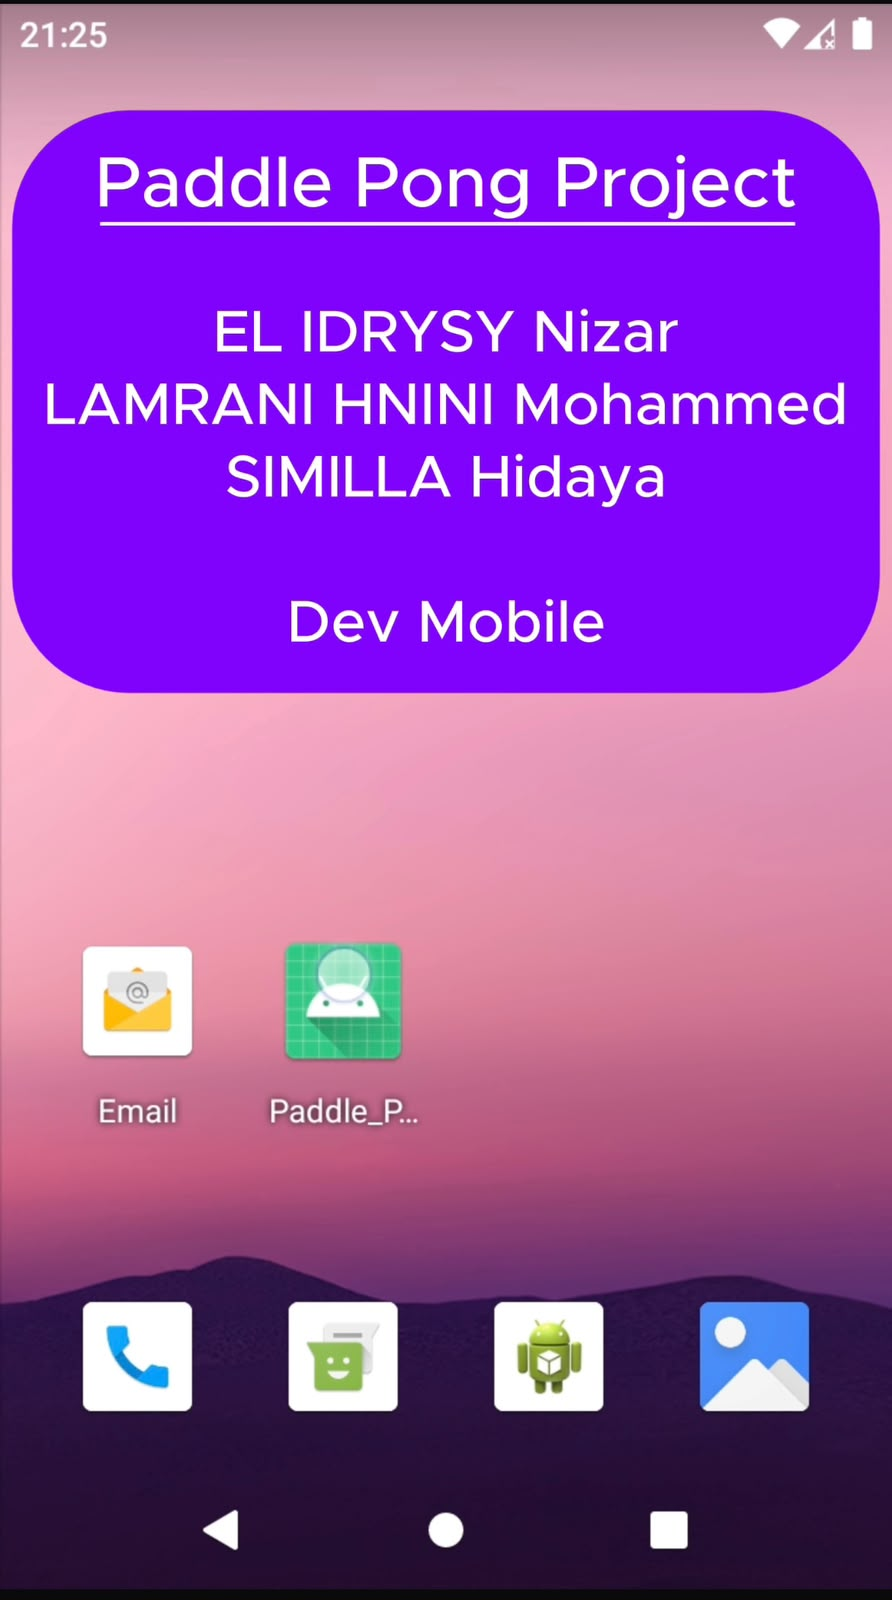
\includegraphics[width=0.38\textwidth]{android_home.png}
    \caption{\'Ecran d'accueil Android montrant l'ic\^one de l'application Paddle Pong avant son lancement.}
    \label{fig:android_home}
\end{figure}

La figure~\ref{fig:main_page_modes} compare l'\'ecran principal de configuration (\textit{Setup Screen}) selon le th\`eme s\'electionn\'e : mode clair (\textit{Light Mode}) et mode sombre (\textit{Dark Mode}).

\begin{figure}[H]
    \centering
    \begin{subfigure}[b]{0.44\textwidth}
        \centering
        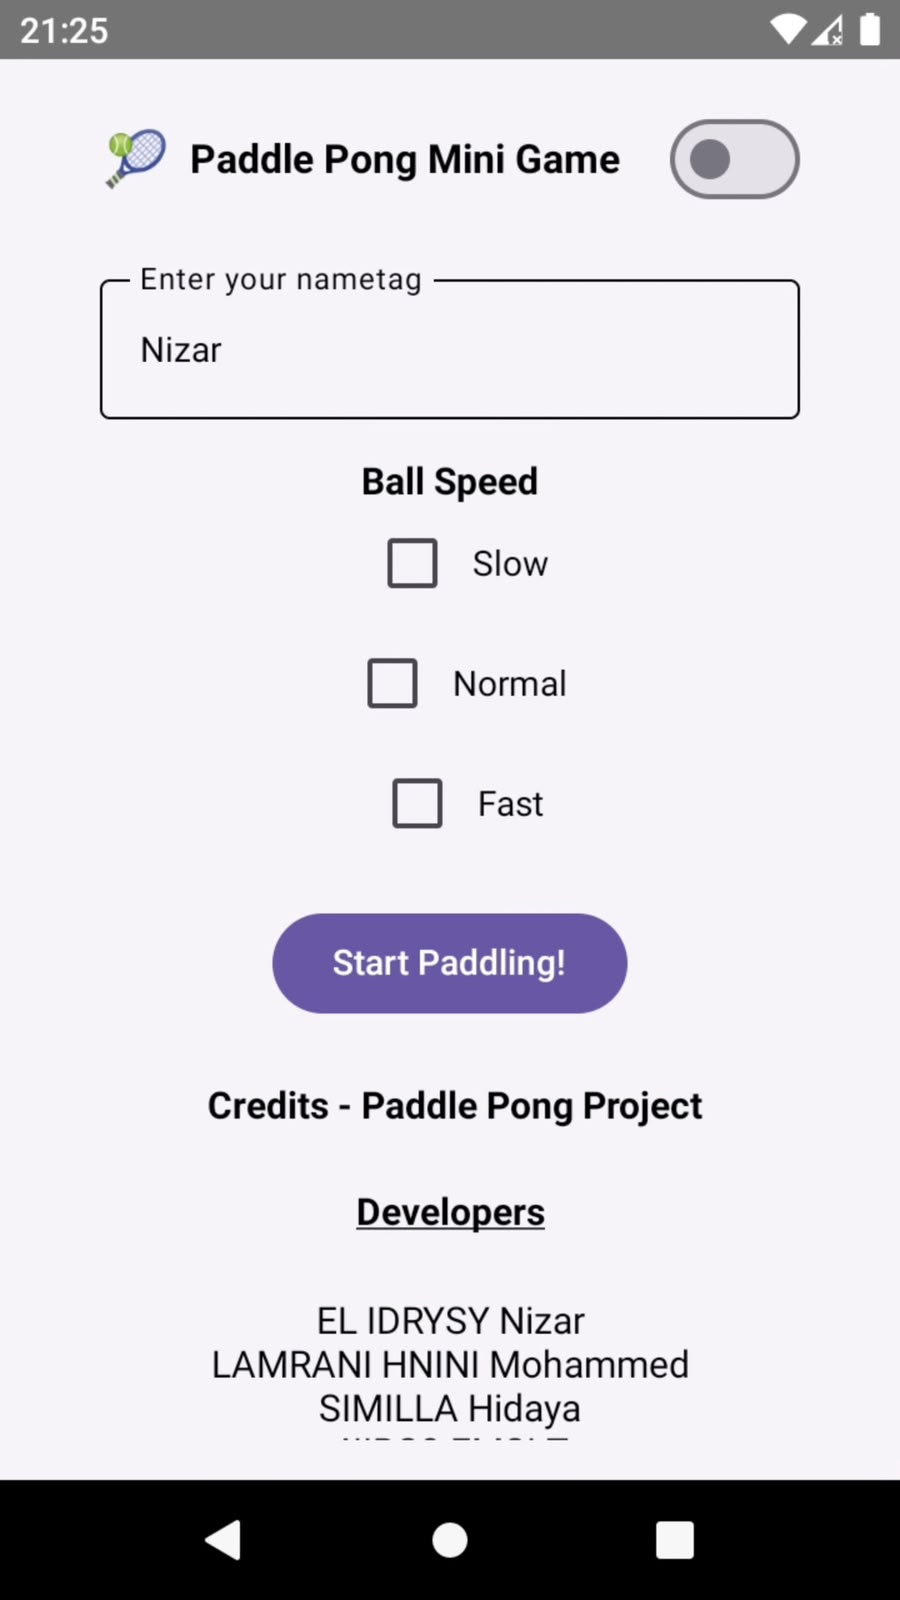
\includegraphics[width=\textwidth]{main_light.png}
        \caption{Page principale en mode clair (\textit{Light Mode}).}
        \label{fig:main_light}
    \end{subfigure}
    \hfill
    \begin{subfigure}[b]{0.44\textwidth}
        \centering
        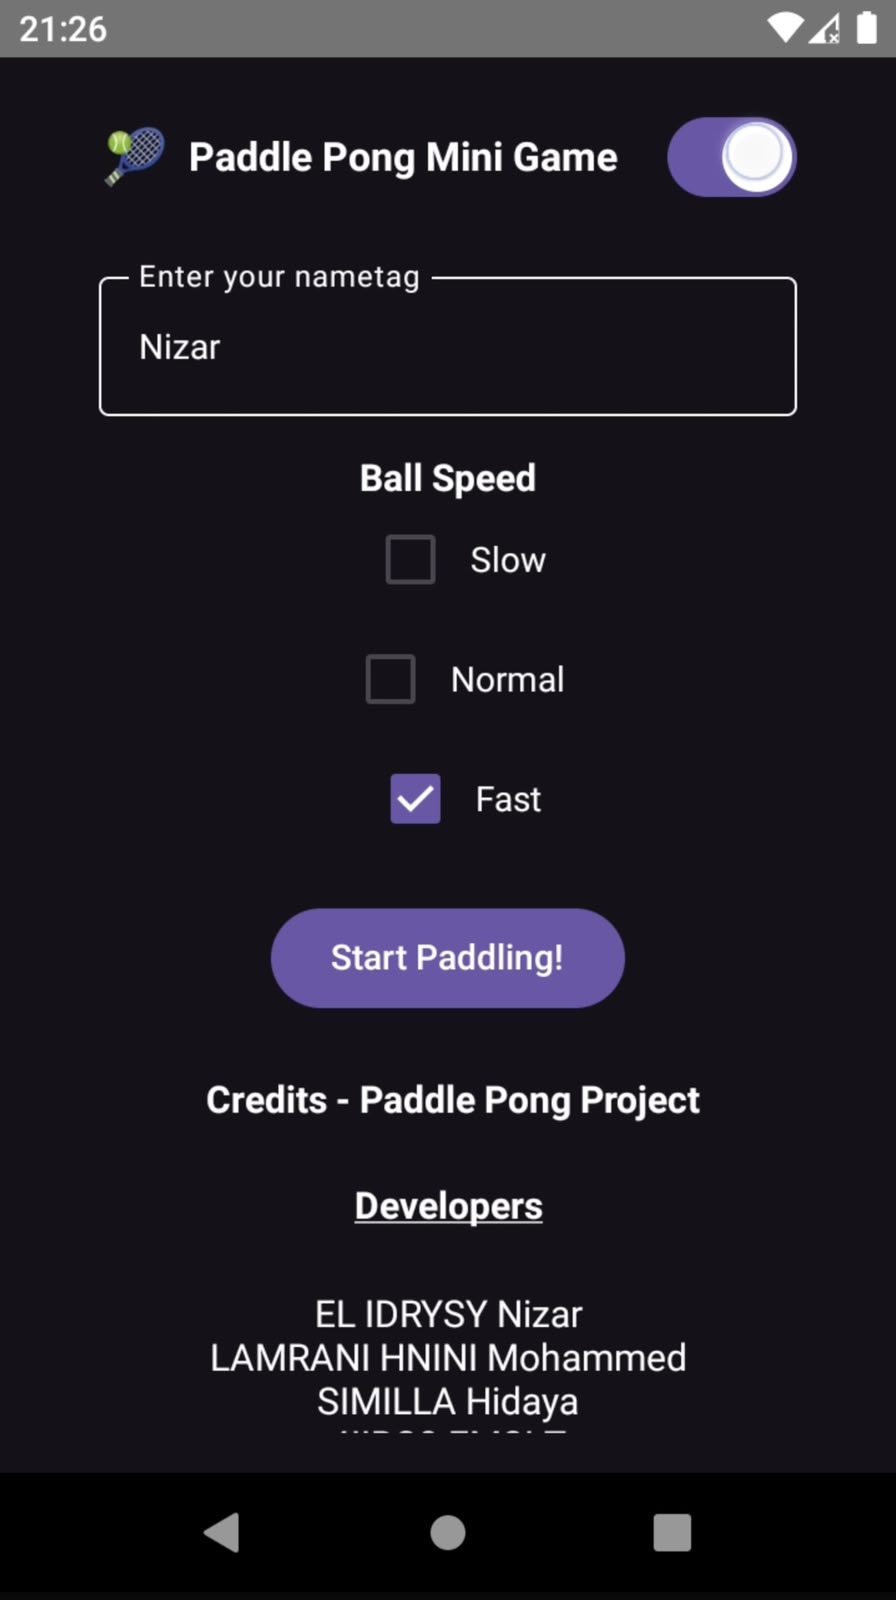
\includegraphics[width=\textwidth]{main_dark.png}
        \caption{Page principale en mode sombre (\textit{Dark Mode}).}
        \label{fig:main_dark}
    \end{subfigure}
    \caption{Comparaison de la page principale de configuration en mode clair et en mode sombre.}
    \label{fig:main_page_modes}
\end{figure}

Enfin, la figure~\ref{fig:game_screen} illustre l'\'ecran de jeu en cours de partie avec le terrain vert, la balle, la raquette rouge, le score et les boutons de contr\^ole.

\begin{figure}[H]
    \centering
    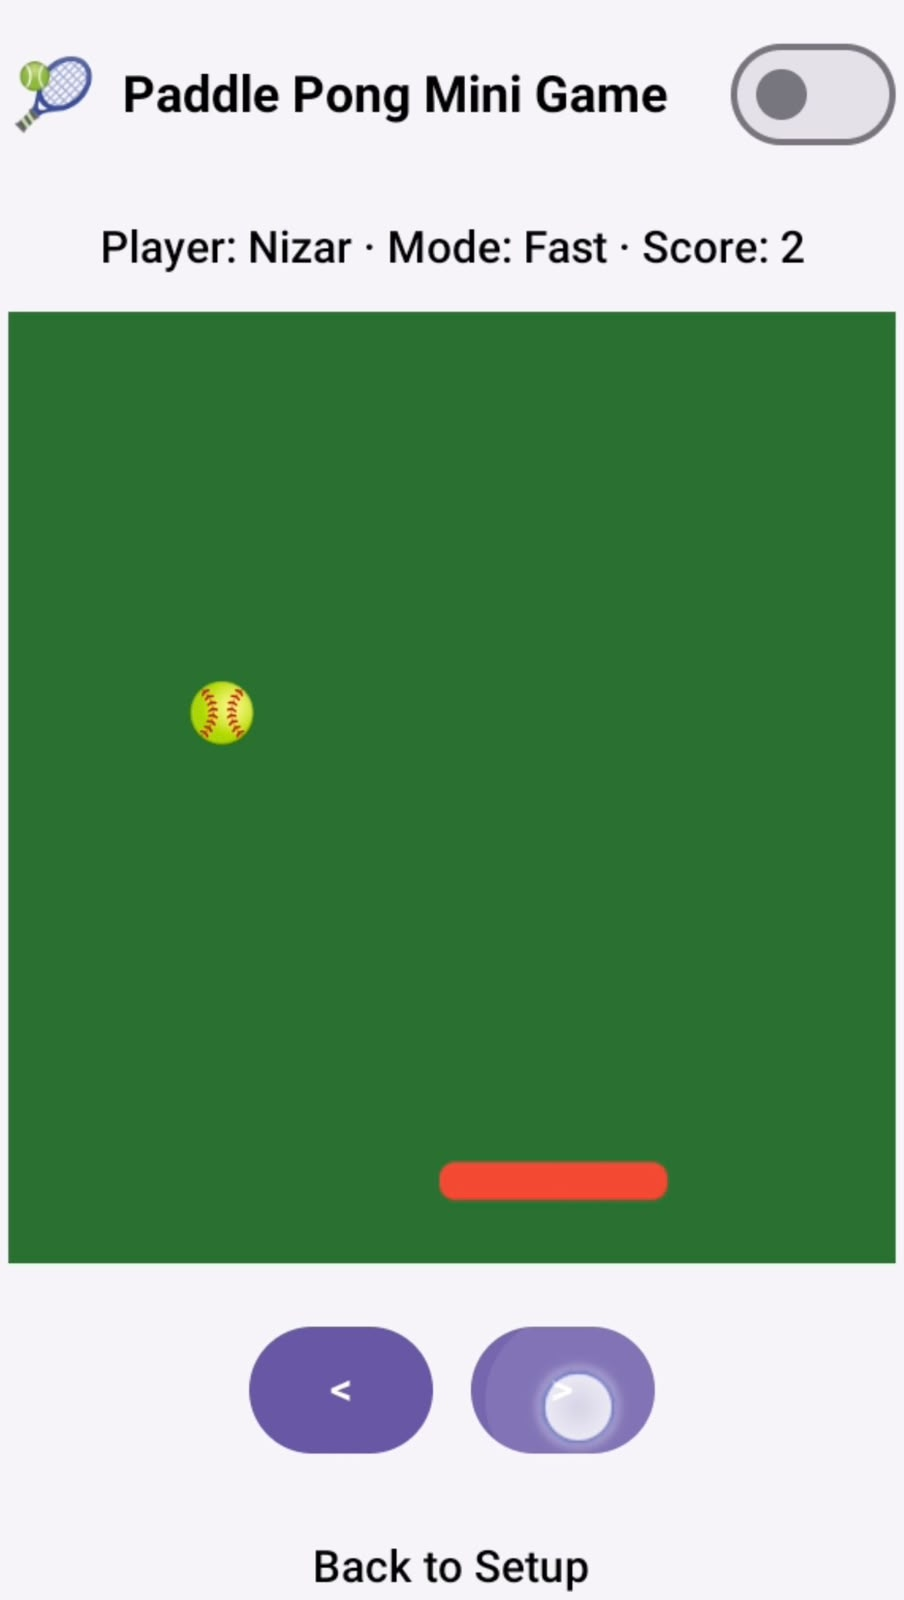
\includegraphics[width=0.38\textwidth]{game_screen.png}
    \caption{\'Ecran de jeu Paddle Pong en cours de partie.}
    \label{fig:game_screen}
\end{figure}

\subsection{Tests fonctionnels}
Les tests fonctionnels ont \'et\'e r\'ealis\'es manuellement sur l'\'emulateur Android (Pixel 5 API 33) et sur un appareil physique. Le tableau~\ref{tab:tests} synth\'etise les sc\'enarios de test ex\'ecut\'es et leurs r\'esultats.

\begin{table}[H]
\centering
\caption{R\'esultats des tests fonctionnels de l'application Paddle Pong}
\label{tab:tests}
\begin{tabularx}{\textwidth}{lXc}
\toprule
\textbf{Sc\'enario de test} & \textbf{R\'esultat attendu} & \textbf{Statut} \\
\midrule
Saisie pseudonyme vide + clic Start & Message d'erreur affich\'e, jeu non lanc\'e & \checkmark \\
Saisie pseudonyme valide + clic Start & Transition vers l'\'ecran de jeu & \checkmark \\
S\'election vitesse Lent & D\'elai de 65 ms appliqu\'e \`a la boucle & \checkmark \\
S\'election vitesse Rapide & D\'elai de 30 ms appliqu\'e \`a la boucle & \checkmark \\
Activation mode sombre & Palette de couleurs sombres appliqu\'ee & \checkmark \\
Rebond balle sur mur gauche & La balle rebondit et repart vers la droite & \checkmark \\
Rebond balle sur mur droit & La balle rebondit et repart vers la gauche & \checkmark \\
Rebond balle sur mur haut & La balle rebondit et repart vers le bas & \checkmark \\
Interception balle par raquette & Score incr\'ement\'e de 1, balle rebondit & \checkmark \\
Balle sort par le bas & AlertDialog Game Over affich\'e & \checkmark \\
Clic ``Play Again?'' & Score remis \`a 0, partie relance\'e & \checkmark \\
Clic ``End Game'' & Retour \`a l'\'ecran de configuration & \checkmark \\
D\'eplacement raquette hors limites gauche & Raquette bloqu\'ee \`a x = 0 & \checkmark \\
D\'eplacement raquette hors limites droite & Raquette bloqu\'ee \`a x = 208 & \checkmark \\
Bouton ``Back to Setup'' en jeu & Retour \`a l'\'ecran de configuration & \checkmark \\
\bottomrule
\end{tabularx}
\end{table}

L'ensemble des 15 sc\'enarios de test ont \'et\'e valid\'es avec succ\`es ($\checkmark$) sur \'emulateur et appareil physique.

\subsection{R\'esultats et discussion --- Matrice SWOT}
La matrice SWOT ci-dessous pr\'esente le bilan diagnostique et strat\'egique du projet Paddle Pong.

\begin{figure}[H]
\centering
\begin{tikzpicture}[font=\scriptsize]
    \draw[darkblue, very thick] (0,0) rectangle (14,-8);
    \draw[darkblue, thick] (7,0) -- (7,-8);
    \draw[darkblue, thick] (0,-4) -- (14,-4);

    \fill[green!30!black] (0,0) rectangle (7,-0.6);
    \fill[red!60!black]   (7,0) rectangle (14,-0.6);
    \fill[blue!60!black]  (0,-4) rectangle (7,-4.6);
    \fill[orange!80!black](7,-4) rectangle (14,-4.6);

    \node[white, font=\bfseries] at (3.5,-0.3) {FORCES (STRENGTHS)};
    \node[white, font=\bfseries] at (10.5,-0.3) {FAIBLESSES (WEAKNESSES)};
    \node[white, font=\bfseries] at (3.5,-4.3) {OPPORTUNIT\'ES (OPPORTUNITIES)};
    \node[white, font=\bfseries] at (10.5,-4.3) {MENACES (THREATS)};

    % Forces
    \node[align=left, text width=6.2cm] at (3.5,-2.2) {
        $\bullet$ Code 100\% Kotlin/Compose moderne.\\
        $\bullet$ Application l\'eg\`ere ($<$1 Mo d'APK logique).\\
        $\bullet$ Interface Material 3 avec mode sombre.\\
        $\bullet$ Game loop non bloquante (coroutines).
    };

    % Faiblesses
    \node[align=left, text width=6.2cm] at (10.5,-2.2) {
        $\bullet$ Pas d'utilisation du Canvas Compose.\\
        $\bullet$ Positionnement par padding (non pixel-perfect).\\
        $\bullet$ Vitesse fixe ($\pm$4 dp) sans acc\'el\'eration.\\
        $\bullet$ Pas de persistance du meilleur score.
    };

    % Opportunites
    \node[align=left, text width=6.2cm] at (3.5,-6.2) {
        $\bullet$ Ajout de niveaux de difficult\'e progressifs.\\
        $\bullet$ Contr\^ole tactile par glissement (drag).\\
        $\bullet$ Tableau des meilleurs scores (Room DB).\\
        $\bullet$ Effets sonores et animations Compose.
    };

    % Menaces
    \node[align=left, text width=6.2cm] at (10.5,-6.2) {
        $\bullet$ Variabilit\'e du rendu selon la densit\'e d'\'ecran.\\
        $\bullet$ Latence possible sur appareils d'entr\'ee de gamme.\\
        $\bullet$ Emoji non uniforme entre fabricants.\\
        $\bullet$ Concurrence de moteurs de jeu d\'edi\'es (Unity).
    };
\end{tikzpicture}
\caption{Matrice d'analyse SWOT du projet Paddle Pong}
\label{fig:swot_analysis}
\end{figure}

La matrice SWOT met en \'evidence la solidit\'e technique de la solution choisie (architecture Compose moderne, game loop asynchrone) tout en identifiant des axes d'am\'elioration concrets pour une version ult\'erieure du jeu, notamment l'adoption du \texttt{Canvas} Compose pour un rendu pixel-perfect et l'ajout de persistance des scores via Room.

\section*{Conclusion}
Ce chapitre a d\'emontr\'e la r\'ealisation technique du projet Paddle Pong, depuis la structure du code source jusqu'aux tests de validation fonctionnelle, en passant par l'analyse critique SWOT du produit livr\'e.

\newpage

% ============================================================
% CONCLUSION ET PERSPECTIVES
% ============================================================
\chapter*{Conclusion et perspectives}
\addcontentsline{toc}{chapter}{Conclusion et perspectives}
\markboth{Conclusion et perspectives}{Conclusion et perspectives}

Le projet \textbf{Paddle Pong}, r\'ealis\'e dans le cadre du module de D\'eveloppement Mobile en 4\textsuperscript{\`eme} ann\'ee du cycle d'ing\'enieur \`a l'EMSI Tanger, a constitu\'e une exp\'erience formatrice et enrichissante, nous permettant de mettre en pratique l'ensemble des comp\'etences acquises en programmation Kotlin et en d\'eveloppement Android moderne.

L'ensemble des objectifs initiaux fix\'es dans le cahier des charges a \'et\'e atteint avec succ\`es. Nous avons con\c{c}u et d\'evelopp\'e une application Android native fonctionnelle, int\'egralement r\'ealis\'ee en \textbf{Jetpack Compose}, embarquant un moteur de jeu 2D bas\'e sur les \textbf{coroutines Kotlin}. L'application propose une exp\'erience de jeu compl\`ete : \'ecran de configuration personnalisable (pseudonyme, vitesse, mode sombre), terrain de jeu avec balle rebondissante et raquette contr\^ol\'ee par le joueur, syst\`eme de score et dialogue de fin de partie. Les 15 sc\'enarios de test fonctionnel ont tous \'et\'e valid\'es sur \'emulateur et appareil physique.

Sur le plan technique, ce projet nous a permis d'approfondir notre compr\'ehension du paradigme d\'eclaratif de Compose, de la gestion d'\'etat r\'eactif avec \texttt{mutableStateOf} et \texttt{remember}, de la programmation asynchrone avec les coroutines et \texttt{LaunchedEffect}, ainsi que de la d\'etection de collisions AABB en 2D. L'analyse SWOT a mis en \'evidence les forces du projet (code moderne, application l\'eg\`ere, interface Material 3) tout en identifiant des faiblesses structurelles (positionnement par padding, absence de Canvas, pas de persistance).

En guise de perspectives d'am\'elioration pour une version ult\'erieure, nous recommandons :
\begin{itemize}
    \item La migration du rendu de jeu vers le composant \textbf{Canvas} de Compose pour un positionnement pixel-perfect et des animations fluides \`a 60 FPS.
    \item L'ajout d'un contr\^ole par \textbf{glissement tactile} (\texttt{Modifier.pointerInput}) pour une ergonomie am\'elior\'ee.
    \item L'impl\'ementation d'un \textbf{tableau des meilleurs scores} persistant via la biblioth\`eque Room (base de donn\'ees SQLite locale).
    \item L'int\'egration d'\textbf{effets sonores} via l'API \texttt{SoundPool} d'Android pour renforcer l'immersion.
    \item L'ajout de \textbf{niveaux de difficult\'e progressifs} avec augmentation dynamique de la vitesse apr\`es chaque palier de score.
    \item Le d\'eploiement sur le \textbf{Google Play Store} pour une diffusion publique.
\end{itemize}

Sur le plan personnel et acad\'emique, ce projet a renforc\'e notre esprit d'\'equipe, notre capacit\'e \`a structurer un projet logiciel de bout en bout (analyse, conception UML, impl\'ementation, tests) et notre passion pour le d\'eveloppement mobile Android.

\newpage

% ============================================================
% BIBLIOGRAPHIE ET WEBOGRAPHIE
% ============================================================
\begin{thebibliography}{99}
\addcontentsline{toc}{chapter}{Bibliographie}

\bibitem{statcounter}
StatCounter. (2026). \textit{Mobile Operating System Market Share Worldwide}. StatCounter Global Stats. \url{https://gs.statcounter.com/os-market-share/mobile/worldwide}

\bibitem{kotlin_android}
Google. (2019). \textit{Kotlin-first approach for Android development}. Android Developers Blog. \url{https://developer.android.com/kotlin/first}

\bibitem{kotlin_coroutines}
JetBrains. (2024). \textit{Kotlin Coroutines Guide}. Kotlin Documentation. \url{https://kotlinlang.org/docs/coroutines-guide.html}

\bibitem{compose_docs}
Google. (2024). \textit{Jetpack Compose Documentation}. Android Developers. \url{https://developer.android.com/jetpack/compose}

\bibitem{android_distribution}
Google. (2024). \textit{Android Platform Distribution Dashboard}. Android Developers. \url{https://developer.android.com/about/dashboards}

\bibitem{game_programming_patterns}
Nystrom, R. (2014). \textit{Game Programming Patterns}. Genever Benning. \url{https://gameprogrammingpatterns.com/game-loop.html}

\bibitem{material3}
Google. (2024). \textit{Material Design 3 -- Design Guidelines}. Material Design. \url{https://m3.material.io/}

\bibitem{compose_state}
Google. (2024). \textit{State and Jetpack Compose}. Android Developers. \url{https://developer.android.com/jetpack/compose/state}

\bibitem{android_studio}
Google. (2024). \textit{Android Studio User Guide}. Android Developers. \url{https://developer.android.com/studio/intro}

\bibitem{compose_side_effects}
Google. (2024). \textit{Side-effects in Compose -- LaunchedEffect}. Android Developers. \url{https://developer.android.com/jetpack/compose/side-effects}

\bibitem{pong_history}
Kent, S. L. (2001). \textit{The Ultimate History of Video Games}. Three Rivers Press. Chapter on Pong and Atari.

\bibitem{kotlin_docs}
JetBrains. (2024). \textit{Kotlin Programming Language Official Documentation}. \url{https://kotlinlang.org/docs/home.html}

\end{thebibliography}

\end{document}
